\documentclass{article}
\usepackage{tikz}
\usepackage{multicol}
\usepackage[margin=1in]{geometry}
\newcommand{\rkt}[2]{\tt #1. #2}

\begin{document}
{
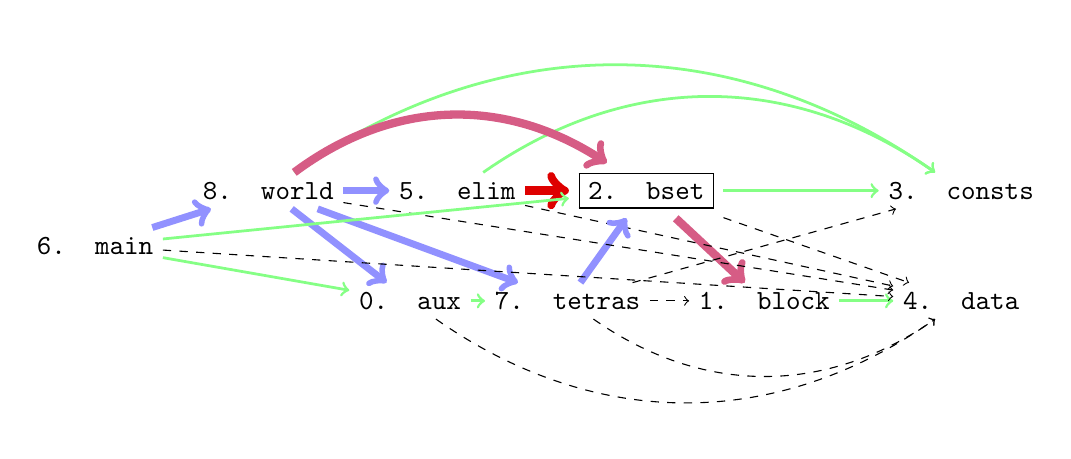
\begin{tikzpicture}

  \node (00)               {\rkt{3}{consts}};
  \node (01) [below of=00,yshift=0.3cm] {};
  \node (02) [below of=01,yshift=0.3cm] {\rkt{4}{data}};

  \node (10) [left of=00,xshift=-1cm] {};
  \node (11) [left of=01,xshift=-1cm] {};
  \node (12) [left of=02,xshift=-1.5cm] {\rkt{1}{block}};

  \node (20) [left of=10,xshift=-1cm] {\fbox{\rkt{2}{bset}}};
  \node (21) [left of=11,xshift=-1cm] {};

  \node (30) [left of=20,xshift=-1.4cm] {\rkt{5}{elim}};
  \node (31) [left of=21,xshift=-1cm] {};
  \node (32) [left of=12,xshift=-1.5cm] {\rkt{7}{tetras}};

  \node (41) [left of=31,xshift=-1cm] {};
  \node (42) [left of=32,xshift=-1cm] {\rkt{0}{aux}};

  \node (50) [left of=30,xshift=-1.4cm] {\rkt{8}{world}};
  \node (51) [left of=41,xshift=-1cm] {};
  \node (52) [left of=42,xshift=-1cm] {};

  \node (61) [left of=51] {\rkt{6}{main}};

  %% -- edges
  %% block
  \draw[->,green!48!white, line width=1pt] (12) -- (02);
  %% bset
  \draw[->,green!48!white, line width=1pt] (20) -- (00);
%% WARNING: no data for boundary 'data.rkt' ==> 'bset.rkt'
  \draw[->,dashed] (20) -- (02);
  \draw[->,purple!64!white, line width=3pt] (20) -- (12);
  %% elim
  \draw[->,green!48!white, line width=1pt] (30) edge[bend left=35] (00);
%% WARNING: no data for boundary 'data.rkt' ==> 'elim.rkt'
  \draw[->,dashed] (30) -- (02);
  \draw[->,red!87!black, line width=3.5pt] (30) -- (20);
  %% tetras
%% WARNING: no data for boundary 'consts.rkt' ==> 'tetras.rkt'
  \draw[->,dashed] (32) -- (00);
%% WARNING: no data for boundary 'data.rkt' ==> 'tetras.rkt'
  \draw[->,dashed] (32) edge[bend right=35] (02);
%% WARNING: no data for boundary 'block.rkt' ==> 'tetras.rkt'
  \draw[->,dashed] (32) -- (12);
  \draw[->,blue!43!white, line width=2.5pt] (32) -- (20);
  %% aux
%% WARNING: no data for boundary 'data.rkt' ==> 'aux.rkt'
  \draw[->,dashed] (42) edge[bend right=35] (02);
  \draw[->,green!48!white, line width=1pt] (42) -- (32);
  %% world
  \draw[->,green!48!white, line width=1pt] (50) edge[bend left=35] (00);
%% WARNING: no data for boundary 'data.rkt' ==> 'world.rkt'
  \draw[->,dashed] (50) -- (02);
  \draw[->,purple!64!white, line width=3pt] (50) edge[bend left=35] (20);
  \draw[->,blue!43!white, line width=2.5pt] (50) -- (30);
  \draw[->,blue!43!white, line width=2.5pt] (50) -- (32);
  \draw[->,blue!43!white, line width=2.5pt] (50) -- (42);
  %% main
%% WARNING: no data for boundary 'data.rkt' ==> 'main.rkt'
  \draw[->,dashed] (61) -- (02);
  \draw[->,green!48!white, line width=1pt] (61) -- (20);
  \draw[->,green!48!white, line width=1pt] (61) -- (42);
  \draw[->,blue!43!white, line width=2.5pt] (61) -- (50);

\end{tikzpicture}}

\begin{verbatim}
Old Runtime: 47027ms

New Runtime: 70ms

Changes:
- Add a typed, wrapping interface to the untyped bset module
  (Remembers that a list is type-checked)

- Change the `tetra` constructor to unwrap output from bset
  (Effected in the adaptor module.)

- Edit the imports of the tetra module to use the new wrapping
  interface instead of directly `(require/typed "bset.rkt" ...)`
\end{verbatim}

\newpage
{
\begin{minipage}{0.4\textwidth}
\begin{verbatim}
;; bset-protector.rkt
#lang typed/racket/base

(require "base-types.rkt" benchmark-util)

(require/typed/check "bset.rkt"
 [blocks-intersect (-> BSet BSet BSet)]
 [blocks-move (-> Real Real BSet BSet)]
 [blocks-rotate-cw (-> Posn BSet BSet)]
 [blocks-rotate-ccw (-> Posn BSet BSet)]
 [blocks-change-color (-> BSet Color BSet)])

(provide (rename-out
 [blocks-intersect+ blocks-intersect]
 [blocks-move+ blocks-move]
 [blocks-rotate-ccw+ blocks-rotate-ccw]
 [blocks-rotate-cw+ blocks-rotate-cw]
 [blocks-change-color+ blocks-change-color]))

(: blocks-intersect+ (-> BSet+ BSet+ BSet+))
(define (blocks-intersect+ b1 b2)
  (wrap
    (blocks-intersect (unwrap b1)
                      (unwrap b2))))

(: blocks-move+ (-> Real Real BSet+ BSet+))
(define (blocks-move+ r1 r2 b1)
  (wrap (blocks-move r1 r2 (unwrap b1))))

(: blocks-rotate-cw+ (-> Posn BSet+ BSet+))
(define (blocks-rotate-cw+ p b)
  (wrap (blocks-rotate-cw p (unwrap b))))

(: blocks-rotate-ccw+ (-> Posn BSet+ BSet+))
(define (blocks-rotate-ccw+ p b)
  (wrap (blocks-rotate-ccw p (unwrap b))))

(: blocks-change-color+ (-> BSet+ Color BSet+))
(define (blocks-change-color+ b c)
  (wrap (blocks-change-color (unwrap b) c)))
\end{verbatim}
\end{minipage}
\hfill
\begin{minipage}{0.4\textwidth}
\begin{verbatim}
;; base-types.rkt (the adaptor)
#lang typed/racket

(require benchmark-util)
(require/typed/check "data.rkt"
  ;; ... truncated
(require/typed 2htdp/image 
  [#:opaque Image image?])

(define-type Color Symbol)
(define-type Posn posn)
(define-type Block block)
(define-type Tetra tetra)
(define-type World world)
(define-type BSet  (Listof Block))

;; === NEW =========================
(struct bset+ ([val : BSet]))

(define-type BSet+ (U BSet bset+))

(: unwrap (-> BSet+ BSet))
(define (unwrap b)
  (if (bset+? b) (bset+-val b) b))

(: wrap (-> BSet+ BSet+))
(define (wrap b)
  (if (bset+? b) b (bset+ b)))

(: make-tetra (-> Posn BSet+ Tetra))
(define (make-tetra a b)
  (tetra a (unwrap b)))
;; === NEW =========================

(provide
 ;; ... truncated
 (rename-out [make-tetra tetra]))
\end{verbatim}
\end{minipage}
}
\end{document}
